\documentclass[11pt]{article}
\usepackage{cite}
\usepackage[a4paper, total={6in, 8in}, margin=0.8in]{geometry}
\usepackage{graphicx}
\graphicspath{ {./assets} }
\title{GAPTCHA}
\author{Logan Lieou}
\date{\today}

\begin{document}
% title page
\maketitle{}
\newpage

\begin{abstract}
   Over the years computer vision has become more and more complex over time, and the ability for companies and websites to prevent botting online has become a more difficult issue. The Completely Automated Public Turing Test to Tell Computers and Humans Apart (CAPTCHA) test was originally invented to overcome this issue but as time goes on it becomes inc. more difficult to prevent bots from bypassing these tests, in this project we attempt to show how one may go about bypassing the CAPTCHA test using AI.
\end{abstract}
\section{Data}
For this project we used data from a publiclly avalible set of CAPTCHA images on kaggle. Each image is $200\times{}50$ with 4 channels, I assume RGB + some sort of mask for CAPTCHA, this is easily fixed with some preprocessing though, mapping $200\times{}50\times{}4$ into an image that is $200\times{}50\times{}1$. A big issue we face with the overall program is the preprocessing and pipelining of data from raw images to information that we can handle with our model and process in order to get adaquate predicitions. Mapping information from string to a tensor is difficult and there are various approches one such approach is from here \cite{a2019}

\begin{verbatim}
   images = sorted(list(map(str, list(data_dir.glob("*.png")))))
   labels = [img.split(os.path.sep)[-1].split(".png")[0] for img in images]
   characters = set(char for label in labels for char in label)
\end{verbatim}
first the author creates a list of images and labels, labels are extracted from image titles.
\begin{verbatim}
   char_to_num = layers.StringLookup(
    vocabulary=list(characters), mask_token=None
   )
   num_to_char = layers.StringLookup(
    vocabulary=char_to_num.get_vocabulary(), 
    mask_token=None, invert=True
   )
\end{verbatim}
then they write a method to map from characters to tensors and tensors to characters, this this is very abstracted and very declarative but the solution is overall better than the the hard code one hot tensor that we ended up implementing this, would hypothetically scale across different types of image information and data and allow for perhaps more flexible models.
\subsection{One Hot Encoding}
One hot encoding is done by creating a matrix comparing across all classes giving 1 if true, 0 if false, in this case it's 1 if a letter is valued, and 0 if it's not. On the model output you would threshold these values in order to get 1 or 0 predictions.
\begin{verbatim}
   ims = [imread("data/train/" + x) for x in os.listdir("data/train/")]
   lbs = [x[:-4] for x in os.listdir("data/train/")]
\end{verbatim}
I start off the same way as in \cite{a2019} with a slightly different aproach and I think my approach is technically slower because they are using collections. I get all labels, and image paths. Next I write the forward mapping:
\begin{verbatim}
   def forward_map(word):
    one_hot_word = np.zeros((len(word), len(symbols)))
    for n, letter in enumerate(word):
        one_hot_word[n][symbols.index(letter)] = 1
    return one_hot_word
\end{verbatim}
this maps a word to a one hot tensor of size $(5, 100)$ both aproaches are hard code restricted to a set of characters, and word length, this is really unfortunate because this has the tendency to hyper fit our model, there's ways around this by writing a more general data pipeline or using bounding boxes to individually classify characters, which may have been a better aproach overall. The reverse mapping:
\begin{verbatim}
   def inverse_map(one_hot_word):
    word = ""
    for i in range(len(one_hot_word)):
        for j in range(len(one_hot_word[0])):
            if one_hot_word[i][j] >= 1.:
                word += symbols[j]
    return word
\end{verbatim}
Takes in a a one hot tensor and outputs a word.

\section{Model}
\subsection{Intutive Explaination}
In this paper I cover my particular model the CRNN architecutre whatever you want to call it as that's what the architecutre most resembles. The model consists of 3 parts the convolutional, recurrent and transcription layer. When you pass an image to the model the convolutional neural network extracts and learns feature mappings, then you pass these the the RNN, in this case and in the case of my model you use a bidirectional LSTM in order to predict on the variable length label sequence LSTMs are very good at retaining and disregarding previous information. \cite{feng2019} 

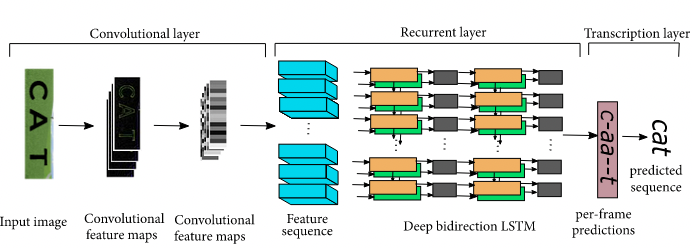
\includegraphics[scale=0.5]{CRNN.png}

\subsection{Mathematical Explaination}
Takes in a Tensor of $(B,C,H,W)$ uses a discrete convolutional function in order to produce feature mappings:
$$
out(N_i, C_{out}) = bias(C_{out}) + \sum_{k=0}^{C_in-1} CCR(weight(C_{out}, k), input(N_i, k))
$$
then down samples after each convolutional block using MaxPool2d:
$$
\mathop{max}_{m=0..kH-1} \mathop{max}_{n=0..kW-1} input(N_i, C_{out},s[0]\times{}h+m, s[1]\times{}w+n)
$$
in order to extract higher level attributes of the image, last takes the convolutional feature maps and maps to feature sequences that can be passed to a bidirectional LSTM to produce sequence predictions that are compared to label forward mappings using $CCE$ loss \cite{pytorch}
LSTMs can be defined as operations on hidden state:
$$i_t = \sigma(W_{ii}x_t + b_{ii} + W_{hi}h_{t-1} + b_{hi})$$
$$f_t = \sigma(W_{if}x_t + b_{if} + W_{hf}h_{t-1} + b_{hf})$$
$$g_t = tanh(W_{ig}x_t + b_{ig} + W_{hg}h_{t-1} + b_{hg})$$
$$o_t = \sigma(W_{io}x_t + b_{io} + W_{ho}h_{t-1} + b_{ho})$$
$$c_t = f_t \circ{} c_{t-1} + i_t \circ{} g_t$$
$$h_t = o_t \circ{} tanh(c_t)$$
``Transcription is used to convert the predictions of each slice made by the Bidirectional LSTM into a label sequence." \cite{feng2019}

\subsection{Code Explaination}
In the code you can see how this architecutre was mapped easily to a tensorflow model. First we want to specify what the shape of our input tensor is in this case:
\begin{verbatim}
   image = layer.Input((1, 50, 200))
\end{verbatim}
where 1 is the number of channels, 50 is the height, and 200 is the width. Next I specify the convolutional layers to produce our feature mappings:
\begin{verbatim}
   out = layers.Conv2D(16, (3, 3), activation="relu", padding="same")(image)
   out = layers.MaxPooling2D((2, 2), padding="same")(out)
   out = layers.Conv2D(32, (3, 3), activation="relu", padding="same")(out)
   out = layers.MaxPooling2D((2, 1), padding="same")(out)
   out = layers.Conv2D(64, (3, 3), activation="relu", padding="same")(out)
   out = layers.MaxPooling2D((2, 5), padding="same")(out)
   out = layers.Conv2D(128, (3, 3), activation="relu", padding="same")(out)
\end{verbatim}
in the case of tensorflow the first arg that is passed specifies the output size in the case of Conv2D it's the number of output channels. Then (3, 3) is the size of the kernel, and MaxPooling2D (2, 2) is the stride specified for the down sampling factor. Next we need to map feature mappings to a feature sequence to be passed to the LSTMs.
\begin{verbatim}
   out = layers.BatchNormalization()(out) # not sure yet
   out = keras.backend.squeeze(out, axis=1)
\end{verbatim}
Now you pass these feature sequences to the LSTM:
\begin{verbatim}
   out = layers.Bidirectional(layers.LSTM(256, return_sequences=True))(out)
   out = layers.Bidirectional(layers.LSTM(256, return_sequences=True))(out) 
\end{verbatim}
256 is the number of output features this is a point where HPO could come in. Once we have the outputs of the LSTM we enter the transcription layer which essentially will output the softmax tensor we can compare to forward\(y\):
\begin{verbatim}
   out = keras.backend.expand_dims(out, axis=2)
   out = layers.Conv2D(len(symbols), (2, 2)
         , activation="relu", padding="same")(out)
   out = keras.backend.squeeze(out, axis=2)
   out = layers.Softmax()(out)
\end{verbatim}
Last with tensorflow you need to compile your model to specify which loss function and optimizer you would like to use in our case we use CCE loss and ADAM optimizer:
\begin{verbatim}
   model.compile(loss="categorical_crossentropy"
      , optimizer="adam")
\end{verbatim}

\section{Loss}
We used categorical cross entropy as well as CTC loss.
\subsection{Categorical Cross Entropy}
Categorical cross entropy is a common loss function when dealing with many catgegories of data to classify cross entropy can be expressed
$$
CE = -\sum_{x\in{}X} f(x)log(g(x))
$$
Cross entropy comes from information theory and measures the the average number of bits from distrobution $g$ reletive to a given distrobution $f$ for the same underlying value $x$ \cite{murphy2012} in the case of binary cross entropy we compare two distrobutions which can be represented as
$$
BCE = -w_n [y_n \dot{} log x_n + (1 - y_n) \dot{} log(1 - x_n)]
$$
Categorical cross entropy simply extrapolates this notion and expands to $n$ distrobutions where each distrobution represents the output of some category.
$$
CCE = -\sum_{c=1}^{C} w_c log \frac{exp(x_{n, c})}{exp(\sum_{i=1}^{C}x_{n,i})} y_{n,c}
$$
This loss function is commonly used for classifying the pixels of a 2D image, or letters in a word.

\subsection{Connectionist Temporal Classification}
CTC was first proposed in \cite{graves2006}

\section{Training}
A simple training function may look something like this:
\begin{verbatim}
   for epoch in range(10):
      for X, y in train_dataset:
         optim.zero_grad()
         preds = model(X)
         loss = loss_fn(preds, y)
         optim.step()
\end{verbatim}
where you take feature inputs and validate these against labels the adjust the model accordingly using your optimizer. The interesting part here is of course the forward and inverse mappings of the data, y must be encoded with the forward mapping then y and model(X) can be compared. Training is simply an optimization problem where we attempt to minimize some loss function.

\section{Problems}
Our models had issues with overfitting, this is due to how preprocessing works as covered before, in addition this also somewhat has to do with the way that tensorflow works as well as a lack of experience and knowledge.
\subsection{Preprocessing}
Preprocssing hard fit the model to only predict a certian length of characters, as well as in some cases only a certian subset of characters, as well although this is very good for our results it's not very good for generalizing the model, you could potentially improve this by having a dataset that contains all characters.

\subsection{Tensorflow}
Writing anything other than a purely sequential model quickly becomes a nightmare, writing custom loops, mappings, etc. is very difficult as keras in particular is based around the layers api, tensors must have a predefined size beforehand, debuging is a difficult especically for beginner, causing us to copy lots of code while not really understanding what it does.

\section{Conclusion}
Datasets could be improved by providing more variation across more symbols, Models can be improved by not hyper fitting to the length of symbols in the dataset, you could do OCR on n symbols using bounding box, this would allow you to identify any length string, and the task would be to calssify a character into 1 of 100 categories instead, of trying to classify into 500 categories or MaxLength*SymbolsLength categories, this could improve accuracy of the model as well as extensibility to other CAPTCHA tests that are not 5 characters or are not constrained to these characters. Possible other approaches could be reinforcement learning showing a model mass amounts of CAPTCHA until it's able to distinguish letters symbols etc. similar to how a human may learn, additionally. We could improve the models that we have by creating more efficent mappings between symbols and tensors, for a smoother more effecive pre process pipeline to work across many different webpages and applications.

\bibliography{paper}{}
\bibliographystyle{ieeetr}
\end{document}